\documentclass{article}
\usepackage{tikz}
\usetikzlibrary{shapes, arrows, positioning}

\begin{document}
	
	\begin{figure}[h]
		\centering
		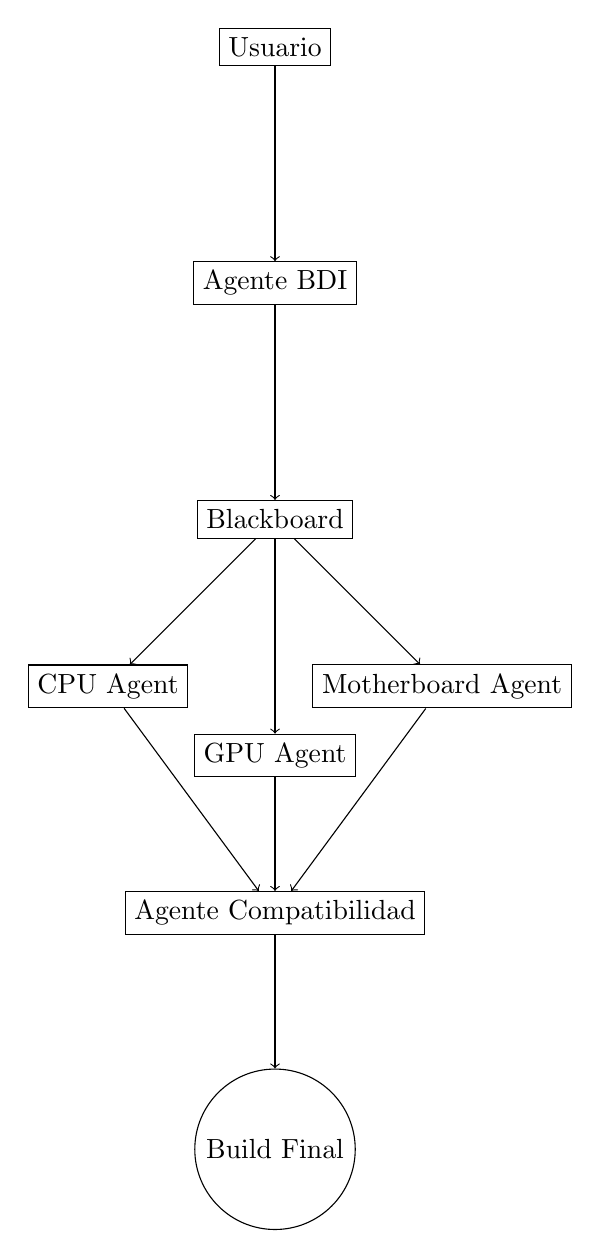
\begin{tikzpicture}[node distance=3cm, auto]
			\node (usuario) [rectangle, draw] {Usuario};
			\node (bdi) [rectangle, draw, below of=usuario] {Agente BDI};
			\node (blackboard) [rectangle, draw, below of=bdi] {Blackboard};
			\node (cpu) [rectangle, draw, below left of=blackboard] {CPU Agent};
			\node (gpu) [rectangle, draw, below of=blackboard] {GPU Agent};
			\node (motherboard) [rectangle, draw, below right of=blackboard] {Motherboard Agent};
			\node (compat) [rectangle, draw, below of=blackboard, yshift=-2cm] {Agente Compatibilidad};
			\node (build) [circle, draw, below of=compat] {Build Final};
			
			\path[->] (usuario) edge (bdi)
			(bdi) edge (blackboard)
			(blackboard) edge (cpu)
			(blackboard) edge (gpu)
			(blackboard) edge (motherboard)
			(cpu) edge (compat)
			(gpu) edge (compat)
			(motherboard) edge (compat)
			(compat) edge (build);
		\end{tikzpicture}
		\caption{Diagrama de arquitectura del sistema}
		\label{fig:arquitectura}
	\end{figure}
	
\end{document}